\documentclass[UTF8,zihao=-4,fontset=windows]{ctexart}

\usepackage[a4paper,margin=2.25cm,headheight=15pt]{geometry}
\usepackage{graphicx}
\usepackage{booktabs}
\usepackage{tabularx}
\usepackage{array}
\usepackage{enumitem}
\usepackage{xcolor}
\usepackage{fancyhdr}
\usepackage{titlesec}
\usepackage{caption}
\usepackage{hyperref}
\usepackage{float}
\usepackage{amsmath}
\usepackage{listings}

\definecolor{navy}{HTML}{000000}
\definecolor{teal}{HTML}{000000}
\definecolor{pale}{HTML}{F3F3F3}
\definecolor{muted}{HTML}{555555}
\definecolor{codebg}{HTML}{F6F6F6}

\hypersetup{colorlinks=true,linkcolor=black,urlcolor=black,citecolor=black,
  pdftitle={自动驾驶技术第二次实验报告},pdfauthor={杜承敖}}
\graphicspath{{assets/}}
\setlength{\parindent}{2em}
\setlength{\parskip}{0.28em}
\setlength{\emergencystretch}{2em}
\renewcommand{\arraystretch}{1.18}
\setcounter{tocdepth}{2}
\captionsetup{font=small,labelfont={bf},skip=6pt}
\setlist[itemize]{leftmargin=2em,itemsep=0.2em,topsep=0.3em}

\lstset{language=Python,basicstyle=\ttfamily\scriptsize,frame=single,
  backgroundcolor=\color{codebg},columns=fullflexible,breaklines=true,
  showstringspaces=false,xleftmargin=0.6em,xrightmargin=0.6em,
  aboveskip=0.45em,belowskip=0.35em}

\titleformat{\section}{\Large\bfseries\color{navy}}{\thesection}{0.7em}{}
\titleformat{\subsection}{\large\bfseries\color{teal}}{\thesubsection}{0.7em}{}
\titlespacing*{\section}{0pt}{1.0em}{0.45em}
\titlespacing*{\subsection}{0pt}{0.7em}{0.3em}

\pagestyle{fancy}
\fancyhf{}
\fancyhead[L]{\small 自动驾驶技术第二次实验}
\fancyhead[R]{\small nuScenes mini 与 PETR 三维检测}
\fancyfoot[C]{\small\color{muted}\thepage}
\renewcommand{\headrulewidth}{0.4pt}


\usepackage{placeins}
\usepackage{needspace}
\lstset{captionpos=b,keepspaces=true,basicstyle=\ttfamily\footnotesize}
\renewcommand{\lstlistingname}{代码清单}
\newcommand{\source}[1]{\par\noindent{\footnotesize\raggedright\textbf{代码位置：}\path{#1}\par}}
\widowpenalty=10000
\clubpenalty=10000
\begin{document}

\begin{titlepage}
  \thispagestyle{empty}
  \begin{center}
    \vspace*{1.8cm}
    {\zihao{1}\bfseries 自动驾驶技术第二次实验报告\par}
    \vspace{1.0cm}
    {\zihao{3}\bfseries nuScenes mini\par}
    \vspace{0.25cm}
    {\zihao{3}\bfseries 多相机三维目标检测与 PETR\par}

    \vfill

    {\zihao{4}
    \renewcommand{\arraystretch}{1.75}
    \begin{tabular}{>{\bfseries}r l}
      姓名： & \underline{\makebox[9.2cm][c]{杜承敖}} \\
      学号： & \underline{\makebox[9.2cm][c]{2024302112019}} \\
      专业： & \underline{\makebox[9.2cm][c]{计算机科学与技术（雷军班）}} \\
      课程： & \underline{\makebox[9.2cm][c]{自动驾驶技术}} \\
    \end{tabular}
    }

    \vfill

    {\zihao{3}\bfseries 武汉大学\par}
    \vspace{0.45cm}
    {\zihao{4}2026 年 9 月 29 日\par}
    \vspace*{0.8cm}
  \end{center}
\end{titlepage}


\pagenumbering{arabic}
\tableofcontents
\clearpage

\phantomsection
\section*{摘要}
\addcontentsline{toc}{section}{摘要}

本报告记录基于 PETR 的多相机三维目标检测实践。实验使用 nuScenes mini 的六路相机数据，将 404 个关键帧按官方场景划分为 323 帧训练数据和 81 帧验证数据。首先结合相机内外参与车辆位姿，将六路相机的图像射线统一到参考自车坐标系进行显示；随后阅读 PETR 的图像特征提取、三维位置编码、Transformer 解码器和集合匹配代码，在 RTX 4060 Laptop GPU 上按教学配置完成 20 轮、6460 次迭代训练。已记录批次的轮平均总损失由 13.408410 降至 8.723793。使用第 20 轮权重对全部 81 帧验证数据进行评估，得到 mAP=0.000569、NDS=0.028768，并按阈值 0.1、每帧 top-20 展示前三帧的六相机图和俯视图。预测框存在明显错位，输出类别高度集中于汽车，说明流程已经完成，但模型尚未具备可靠的三维检测能力。报告中的数值、日志和图像均来自本次实际运行。

\noindent\textbf{关键词：}nuScenes mini；六路相机；统一坐标系；PETR；三维目标检测

\clearpage
\section{实验任务与完成链路}

本次实验按照课程《PETR实践指导文档》开展，沿着“相机数据与标定---统一坐标---特征和位置编码---集合预测---训练与评估”的链路记录实验。与实验一的二维 YOLO 检测不同，本次网络从六路图像直接预测统一三维空间内的目标类别、中心、尺寸、朝向和速度。

本报告覆盖三项主要任务：
\begin{itemize}
  \item 显示六路相机数据在统一自车坐标系中的几何关系，说明内参、外参和不同传感器时间戳位姿的作用；
  \item 记录真实训练 Log、20 轮 Loss 曲线、最终权重、全部验证帧指标和三帧预测可视化；
  \item 结合本地代码理解 PETR 的特征提取、三维位置编码、查询与解码器、匈牙利匹配、损失及输出解码。
\end{itemize}

实验采用课程单帧 PETRv1 配置，不输入点云或历史 sweeps。教学模型使用缩小的分辨率、查询数和解码器层数；实验目的为完成流程和理解实现，不以论文精度作为验收门槛。

\section{数据组织、划分与运行环境}
\Needspace{5\baselineskip}
\subsection{六路图像和 nuScenes 索引}

原始元数据通过 token 关联场景、关键帧、相机文件、标定、车辆位姿与三维标注。\texttt{sample\_annotation} 的真实框位于全局坐标系，\texttt{calibrated\_sensor} 给出传感器标定，\texttt{ego\_pose} 给出车辆位姿。\texttt{preprocess.py} 调用课程转换器，把图片路径、相机参数和真实框整理为训练与验证索引。

\begin{table}[H]
\centering
\caption{本次 nuScenes mini 数据及检查结果}
\begin{tabularx}{\textwidth}{p{4.0cm}Xr}
\toprule
项目 & 内容 & 数量 \\
\midrule
场景 / 关键帧 & 完整 mini 元数据 & 10 / 404 \\
训练划分 & 8 个官方训练场景 & 323 帧 \\
验证划分 & 2 个官方验证场景 & 81 帧 \\
关键帧相机图片 & 每帧六路，所有路径均存在 & 2424 张 \\
样本与场景隔离 & 两组 token 和场景均无重叠 & 已通过 \\
\bottomrule
\end{tabularx}
\end{table}

六路通道为 CAM\_FRONT\_LEFT、CAM\_FRONT、CAM\_FRONT\_RIGHT、CAM\_BACK\_LEFT、CAM\_BACK 和 CAM\_BACK\_RIGHT。本课程包未提供 LiDAR 原始点云，本次仅使用相机图像。代码中使用 LiDAR 坐标系作为共同三维参考，并不等于读取 LiDAR 数据。

\begin{table}[H]
\centering
\caption{训练与验证索引中的十类有效标注数量}
\label{tab:class-counts}
\begin{tabular}{lrr}
\toprule 类别 & 训练集 & 验证集 \\
\midrule
car & 4082 & 2056 \\
truck & 451 & 122 \\
bus & 337 & 41 \\
trailer & 59 & 0 \\
construction\_vehicle & 174 & 0 \\
pedestrian & 3068 & 1260 \\
motorcycle & 179 & 233 \\
bicycle & 147 & 44 \\
traffic\_cone & 773 & 37 \\
barrier & 1851 & 0 \\
\bottomrule
\end{tabular}
\end{table}

表\ref{tab:class-counts}统计 \texttt{valid\_flag=True} 的标注，尚未应用训练范围或评估器距离过滤，不等同于评估器的真实框数量。验证集的 trailer、construction\_vehicle 和 barrier 缺少有效标注，mini 的类别覆盖并不完整。

\Needspace{5\baselineskip}
\subsection{独立环境与训练前检查}

本次新建独立 Conda 环境 \texttt{petr-mini}，保留原有 \texttt{d2l}。安装完成后验证 CUDA、PETR 插件和 DCNv2 CUDA 前向、反向计算；这些属于训练前检查。Python 3.8 的 HTTPS 握手在本机失败，因此将官方安装包通过可联网的下载工具缓存后离线安装，核对 PyTorch 与 torchvision 的官方 SHA256。此方法解决安装问题，不表示 Python HTTPS 问题已经消失。

\begin{table}[H]
\centering
\caption{本次实际运行环境}
\begin{tabularx}{\textwidth}{p{5.2cm}X}
\toprule 项目 & 版本或配置 \\
\midrule
Python & 3.8.19 \\
GPU & NVIDIA GeForce RTX 4060 Laptop GPU \\
GPU 显存 & 8187 MiB \\
PyTorch / torchvision & 1.13.1+cu117 / 0.14.1+cu117 \\
CUDA runtime / OpenSSL & 11.7 / 3.0.18 \\
mmcv-full / mmdet & 1.7.0 / 2.28.2 \\
mmdetection3d / mmseg & 1.0.0rc6 / 0.30.0 \\
\bottomrule
\end{tabularx}
\end{table}
\FloatBarrier

\section{六路相机在统一坐标系下的显示}
\Needspace{5\baselineskip}
\subsection{坐标变换与时间戳补偿}

显示样本选取时间排序后的第 0 个验证帧，场景为 \texttt{scene-0103}。统一显示采用该帧参考 LiDAR 时间戳对应的自车坐标系：$x$ 向前、$y$ 向左、$z$ 向上，单位米。像素 $(u,v)$ 在给定相机光轴深度 $d$ 时对应候选三维点：
\[
\mathbf p_C=dK^{-1}[u,v,1]^{\mathsf T}.
\]
六路相机分别使用各自的内参 $K$ 和外参。考虑相机时间戳 $t_C$ 与参考时间戳 $t_L$ 不完全一致，转换链路为：
\[
\mathbf p_{E(t_L)}=
T_{E(t_L)\leftarrow G}
T_{G\leftarrow E(t_C)}
T_{E(t_C)\leftarrow C}\mathbf p_C.
\]
课程索引中的 \path{sensor2lidar_rotation/translation} 已实现“相机---当时自车---全局---参考自车---LiDAR”链路；本次显示再将参考 LiDAR 坐标转换至参考自车坐标。程序同时用上述独立链路核对六路变换，并将候选点回投影到原图像核对像素位置，检查均通过。

\Needspace{5\baselineskip}
\subsection{统一图像平面、相机位置和视锥}

图\ref{fig:unified-images}把六张真实相机图像置于各自光轴深度 8 m 的虚拟图像平面，并显示到同一自车坐标系。图\ref{fig:unified-bev}显示相机原点、光轴和视锥截面的俯视投影。二者来自同一个实际标定记录，为保证打印可读性，将原始组合图的左右面板分别排版。

\textbf{8 m 是绘图设定的候选深度。}这些图像平面不代表真实物体表面，也不是点云重建。它们用于展示相机标定关系和像素射线方向；PETR 的位置编码在每条射线上使用多个深度候选。

\begin{figure}[H]
\centering
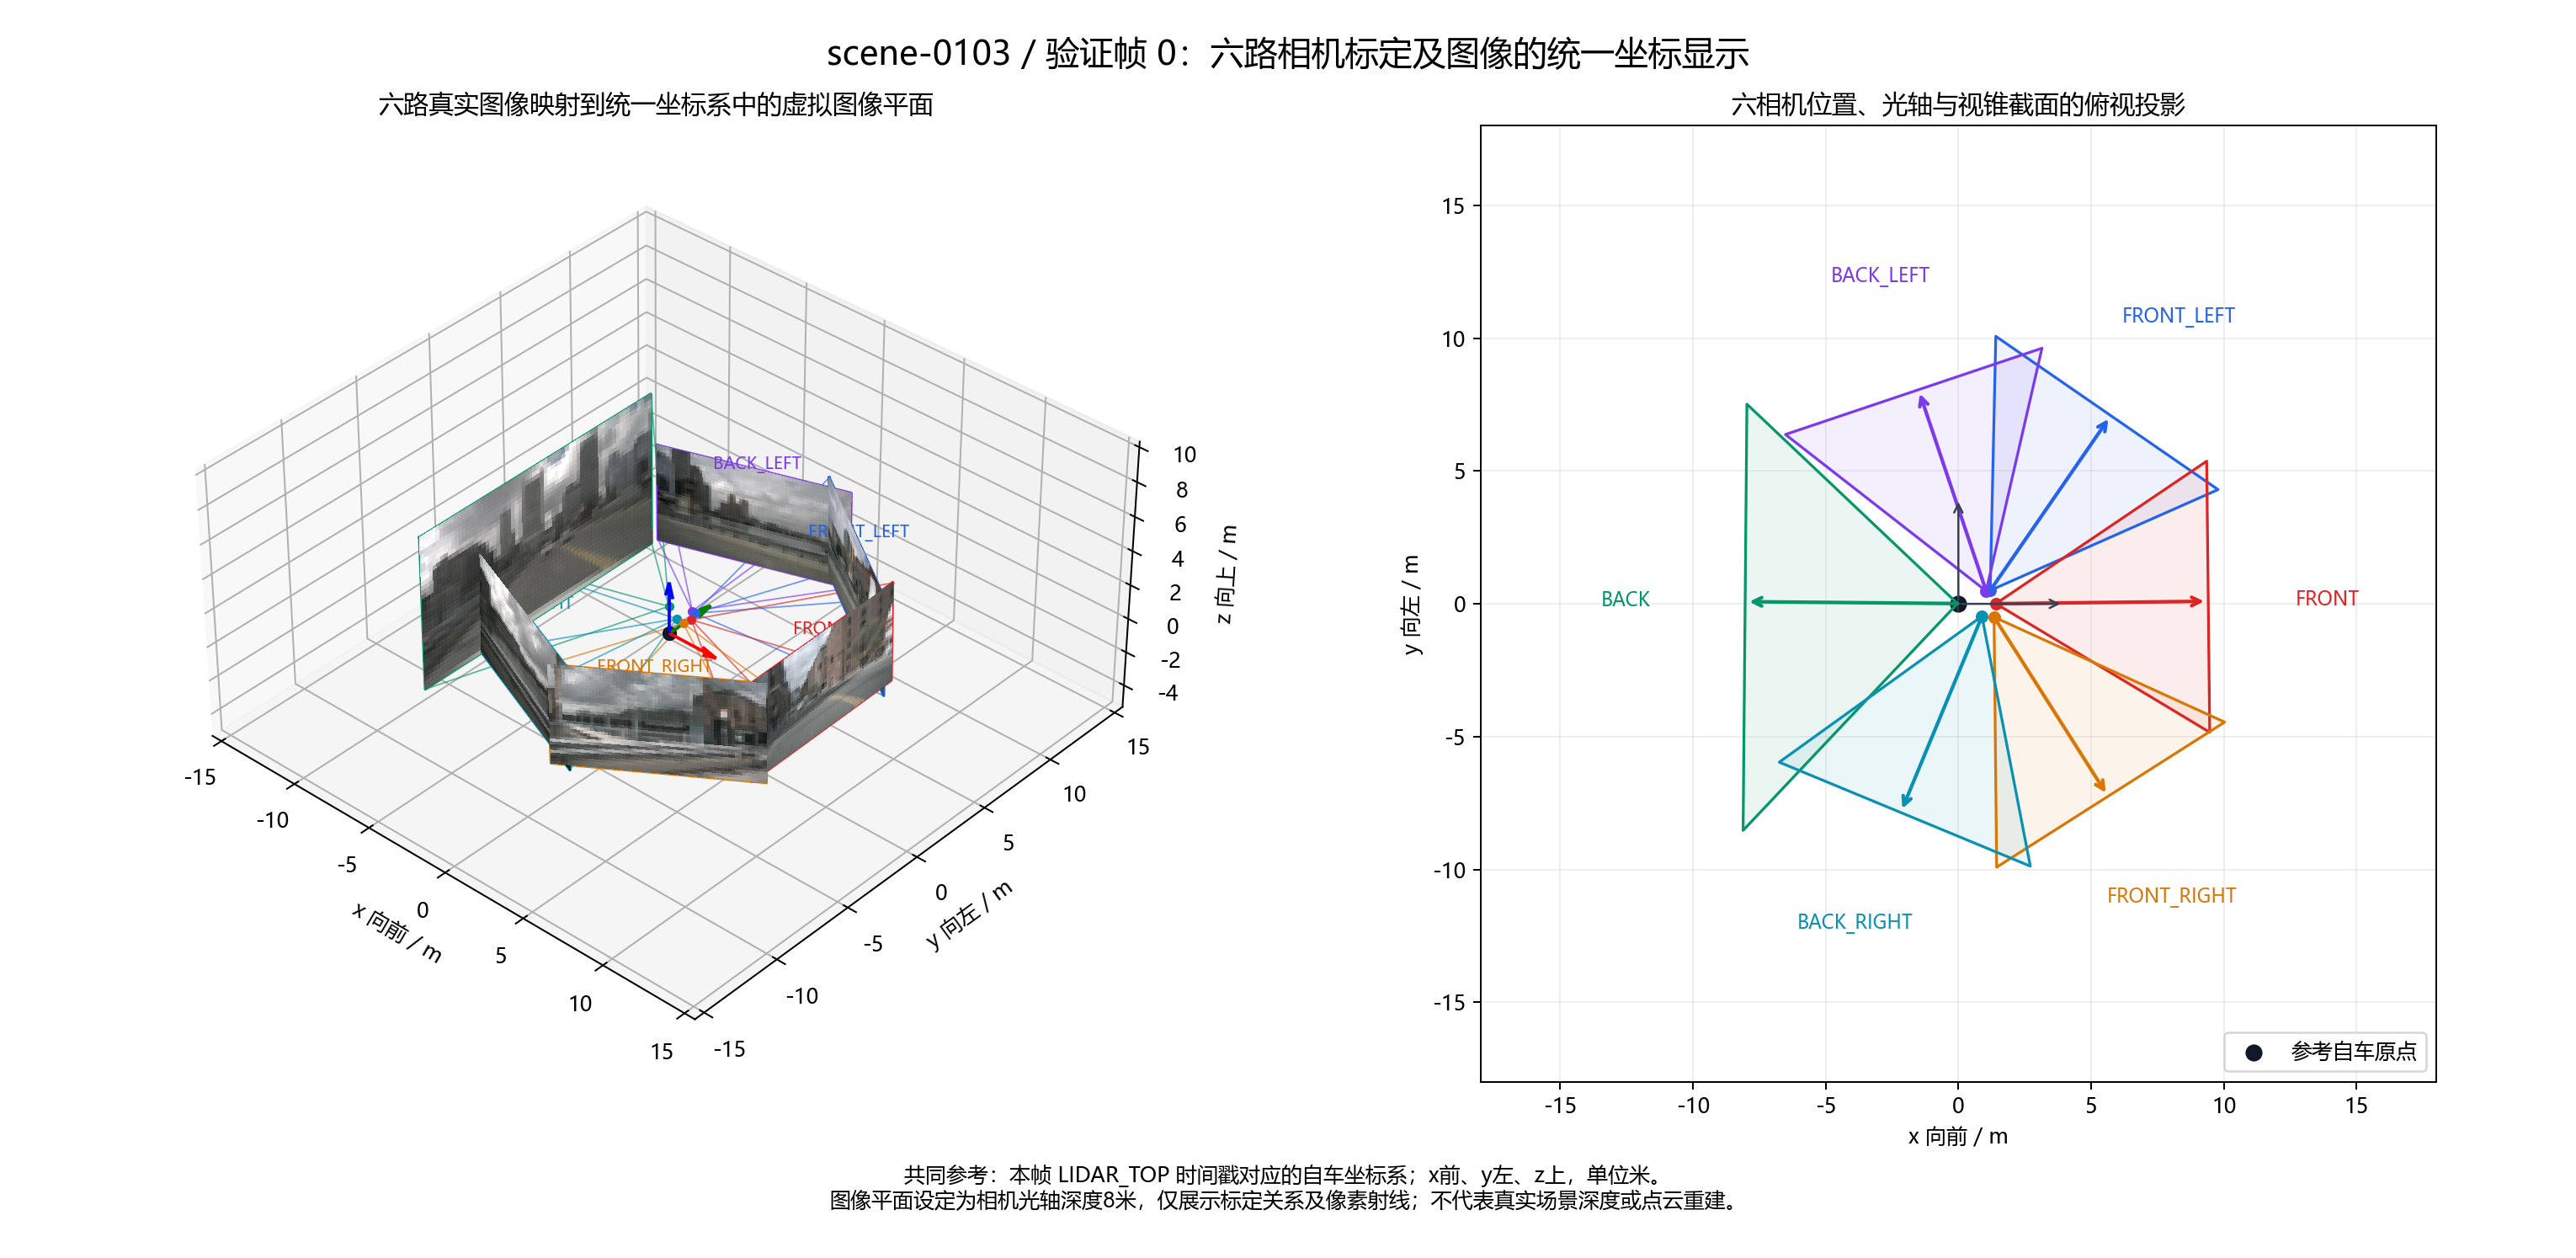
\includegraphics[width=0.88\textwidth,trim=0 50bp 612bp 60bp,clip]{six_camera_unified_coordinates.png}
\caption{六路实际图像及标定视锥在参考自车坐标系中的显示。图像平面设在相机光轴深度 8 m，坐标单位为米。}
\label{fig:unified-images}
\end{figure}

\begin{figure}[H]
\centering
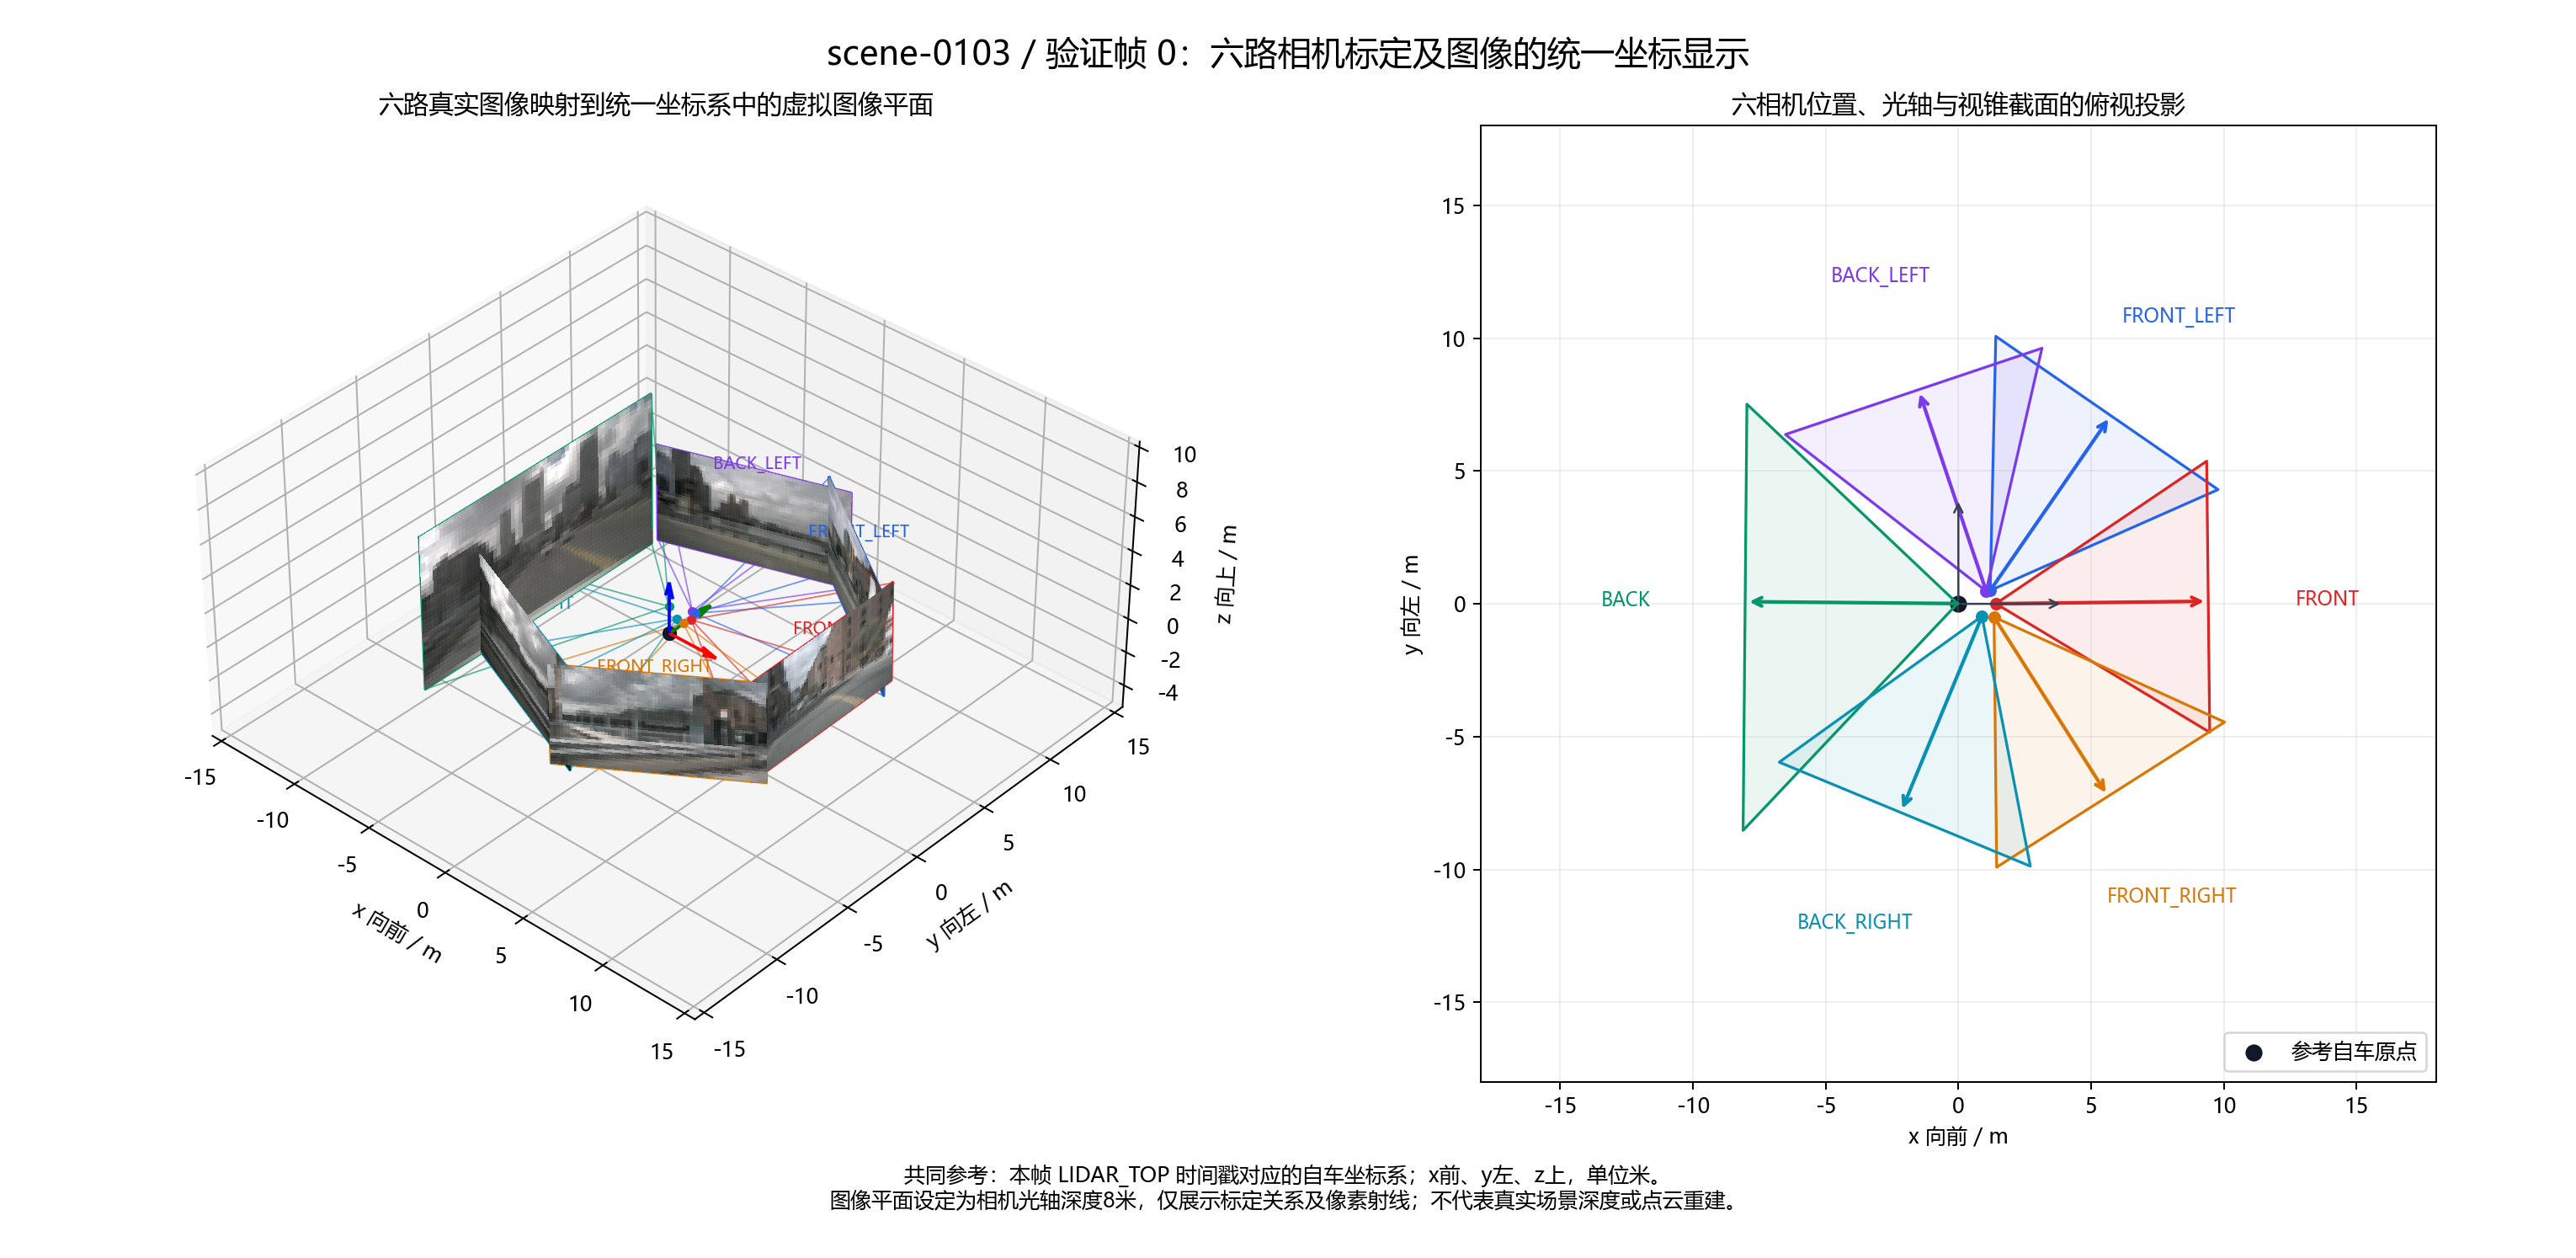
\includegraphics[width=0.80\textwidth,trim=612bp 50bp 0 60bp,clip]{six_camera_unified_coordinates.png}
\caption{六相机的共同坐标俯视显示。彩色点是相机原点，箭头为光轴方向，彩色三角形为视锥截面投影；黑点为参考自车原点。}
\label{fig:unified-bev}
\end{figure}

\begin{table}[H]
\centering
\caption{实际转换到参考自车坐标系的六相机原点}
\begin{tabular}{lrrr}
\toprule 相机 & $x$/m & $y$/m & $z$/m \\
\midrule
CAM\_FRONT\_LEFT & 1.200 & 0.503 & 1.500 \\
CAM\_FRONT & 1.414 & 0.007 & 1.488 \\
CAM\_FRONT\_RIGHT & 1.344 & -0.498 & 1.512 \\
CAM\_BACK\_LEFT & 1.047 & 0.483 & 1.562 \\
CAM\_BACK & -0.033 & 0.011 & 1.566 \\
CAM\_BACK\_RIGHT & 0.889 & -0.466 & 1.547 \\
\bottomrule
\end{tabular}
\end{table}

完整内参、旋转矩阵、时间戳和源图片路径记录在 \path{six_camera_calibration.json}。该坐标显示以参考 LiDAR 时间戳为基准；后文检测俯视图按课程测试脚本使用前相机时刻自车位姿，二者的参考时刻需要分别注明。
\FloatBarrier

\clearpage
\section{PETR 原理与代码理解}
\Needspace{5\baselineskip}
\subsection{入口与图像特征提取}

课程入口调用链为 \texttt{train.py}、框架训练工具、\texttt{Petr3D} 和 \texttt{PETRHead}。网络输入形状为 $[B,6,3,192,512]$，本次 $B=1$。\texttt{Petr3D.extract\_img\_feat} 临时合并 batch 与相机维，使六张图像共享 ResNet50/DCNv2 骨干；经过 CPFPN 后恢复相机维，得到 $[B,6,256,H',W']$ 特征。当前检测头使用第一层特征。代码中名称 \texttt{pts\_bbox\_head} 沿用三维检测框架接口，输入实际为图像特征。

\par\noindent\begin{minipage}{\linewidth}
\source{PETR-official/projects/mmdet3d_plugin/models/detectors/petr3d.py:53}
\begin{lstlisting}[caption={图像特征按相机维恢复，摘录自实际模型}]
img_feats = self.img_backbone(img)
img_feats = self.img_neck(img_feats)
for img_feat in img_feats:
    BN, C, H, W = img_feat.size()
    img_feats_reshaped.append(img_feat.view(B, int(BN / B), C, H, W))
\end{lstlisting}
\end{minipage}\par

\Needspace{5\baselineskip}
\subsection{相机逆投影与三维位置编码}

数据集将相机内参扩成 $4\times4$ 矩阵，与 LiDAR 到相机外参组合为 \texttt{lidar2img}。图像缩放、裁剪后须同步更新内参和该投影矩阵，否则图像特征与三维候选位置无法对应。

\texttt{PETRHead.position\_embeding} 为特征网格建立 $(u,v,d)$ 候选点。配置 \texttt{LID=True}、\texttt{depth\_num=32}，深度按 $d_i=d_0+\Delta i(i+1)$ 非等距采样。再将候选点写为 $(ud,vd,d,1)$，乘 \texttt{lidar2img} 的逆矩阵，得到共同 LiDAR 坐标系中的点。

\par\noindent\begin{minipage}{\linewidth}
\source{PETR-official/projects/mmdet3d_plugin/models/dense_heads/petr_head.py:282}
\begin{lstlisting}[caption={逆投影与位置嵌入；摘录省略维度展开和范围归一化}]
img2lidar.append(np.linalg.inv(img_meta['lidar2img'][i]))
coords3d = torch.matmul(img2lidars, coords).squeeze(-1)[..., :3]
# Normalize xyz to position_range, then rearrange depth as channels.
coords3d = inverse_sigmoid(coords3d)
coords_position_embeding = self.position_encoder(coords3d)
\end{lstlisting}
\end{minipage}\par

每条像素射线的 $32\times3$ 个坐标排列为通道，经位置编码网络映射为 256 维向量，再加多视角正弦位置编码，使注意力能够同时使用外观与几何信息。候选深度不是真实深度标签，网络也不需要先输入真实三维框才能推理。\texttt{position\_range} 控制位置编码范围，\texttt{pc\_range} 控制预测中心映射，两者在本配置中不同。

实现细节上，位置函数计算了越界坐标掩码，但当前 \texttt{forward} 丢弃此返回掩码，注意力继续使用图像 padding masks；因此不能把“计算越界掩码”直接解释为“已进行越界注意力过滤”。

\Needspace{5\baselineskip}
\subsection{共同 memory、查询与三层解码器}

六路特征展平为长度 $6H'W'$ 的共同 memory。100 个可学习三维参考点经过正弦编码及查询网络生成 query embedding；query 内容初始化为零。解码器先以 self-attention 建立查询间关系，再以 cross-attention 读取带三维位置的图像特征，随后经过前馈网络和归一化。每层含 8 个注意力头，本次返回三层中间输出。

\par\noindent\begin{minipage}{\linewidth}
\source{PETR-official/projects/mmdet3d_plugin/models/utils/petr_transformer.py:91}
\begin{lstlisting}[caption={将六路特征展平为统一 memory}]
memory = x.permute(1, 3, 4, 0, 2).reshape(-1, bs, c)
pos_embed = pos_embed.permute(1, 3, 4, 0, 2).reshape(-1, bs, c)
target = torch.zeros_like(query_embed)
\end{lstlisting}
\end{minipage}\par

分类分支输出十类分数；回归分支输出中心、尺寸、朝向和速度的编码。中心偏移与参考点在 inverse-sigmoid 空间相加，sigmoid 后映射到物理范围。框属性编码为 $(c_x,c_y,\log w,\log l,c_z,\log h,\sin\theta,\cos\theta,v_x,v_y)$；解码尺寸用 exp，角度用 $\operatorname{atan2}(\sin\theta,\cos\theta)$。函数 \texttt{normalize\_bbox} 的含义是转换回归表示，并非把全部属性压到 $[0,1]$。

\source{PETR-official/projects/mmdet3d_plugin/core/bbox/util.py:38}

\Needspace{5\baselineskip}
\subsection{匈牙利匹配与损失}

集合预测没有预先指定某个 query 负责某个物体。匹配器计算分类和框回归代价，再使用 \texttt{linear\_sum\_assignment} 一对一分配预测与真实框；没有匹配真实目标的查询作为背景。

\par\noindent\begin{minipage}{\linewidth}
\source{PETR-official/projects/mmdet3d_plugin/core/bbox/assigners/hungarian_assigner_3d.py:116}
\begin{lstlisting}[caption={匹配代价的实际计算}]
cls_cost = self.cls_cost(cls_pred, gt_labels)
normalized_gt_bboxes = normalize_bbox(gt_bboxes, self.pc_range)
reg_cost = self.reg_cost(bbox_pred[:, :8], normalized_gt_bboxes[:, :8])
cost = cls_cost + reg_cost
\end{lstlisting}
\end{minipage}\par

本次分类使用 sigmoid FocalLoss，权重 2.0，$\gamma=2$、$\alpha=0.25$；框回归使用 L1Loss，权重 0.25；GIoULoss 权重为零。日志中 \path{loss_cls/loss_bbox} 对应最后一层，\texttt{d0.*} 和 \texttt{d1.*} 为前两层辅助监督，总 loss 汇总已经加权的六个分量。它不是单独的米制位置误差。

\source{PETR-official/projects/mmdet3d_plugin/models/dense_heads/petr_head.py:701}

\Needspace{5\baselineskip}
\subsection{NMS-free 输出与绘图筛选}

\texttt{NMSFreeCoder.decode\_single} 对 sigmoid 类别分数展平后选取 top-100 的 query/类别组合，按中心范围过滤并还原框属性，没有调用传统 IoU NMS。数据集再将 LiDAR 框转换至自车、全局坐标，生成 nuScenes 格式。绘图脚本在评估之后以阈值 0.1、每帧 top-20 筛选展示框，筛选只影响显示，不改变原始预测或指标。

\source{PETR-official/projects/mmdet3d_plugin/core/bbox/coders/nms_free_coder.py:62}
\FloatBarrier

\clearpage
\section{训练设置、Log 与 Loss 曲线}
\Needspace{5\baselineskip}
\subsection{教学配置和实际命令}

\begin{table}[H]
\centering
\caption{本次训练参数}
\begin{tabularx}{\textwidth}{p{5.2cm}X}
\toprule 参数 & 设置 \\
\midrule
图像 / batch / 精度 & 六路 $192\times512$ / 1 / FP32 \\
骨干与初始化 & ResNet50/DCNv2、CPFPN，公开 ResNet50 权重 \\
查询 / 深度采样 / 解码层 & 100 / 32 / 3 \\
优化器 & AdamW，基础学习率 0.0002，weight decay=0.01 \\
骨干学习率 / 梯度裁剪 & 基础学习率的 0.1 倍 / max\_norm=35 \\
学习率策略 / 随机种子 & CosineAnnealing / 42 \\
训练轮数 / 数据线程 & 20 / workers=0 \\
\bottomrule
\end{tabularx}
\end{table}

本次从课程根目录执行如下命令，结果目录为 \path{outputs/run20}。最终权重 \path{epoch_20.pth} 元数据记录 20 轮、6460 次迭代，浮点权重可加载且全部为有限值。训练阶段不自动做逐轮验证。

\par\noindent\begin{minipage}{\linewidth}
\begin{lstlisting}[language={},caption={本次实际运行命令}]
conda activate petr-mini
cd /d D:\code\autodrive\stage02\PETR
python preprocess.py
python train.py --epochs 20 --work-dir outputs/run20
python test.py --checkpoint outputs/run20/epoch_20.pth
\end{lstlisting}
\end{minipage}\par

再次训练应选择新的空目录。本次未中断；若需从完整 \path{epoch_N.pth} 恢复，\texttt{--epochs 20} 表示最终总轮数，必须使用新的 \texttt{--work-dir}，测试和报告使用实际生成 \path{epoch_20.pth} 的目录。例如：
\par\noindent\begin{minipage}{\linewidth}
\begin{lstlisting}[language={},caption={断点恢复示例，本次未执行}]
python train.py --resume-from outputs/run20/epoch_12.pth --epochs 20 --work-dir outputs/run20_resume
\end{lstlisting}
\end{minipage}\par

\Needspace{5\baselineskip}
\subsection{实际日志与损失变化}

训练循环从 2026-09-29 15:31:17 开始，16:15:41 保存最终权重，约 44.4 分钟。下面摘自本次训练 Log，按可读性保留时间、批次、学习率和损失字段；完整日志仍保存在运行目录。

\par\noindent\begin{minipage}{\linewidth}
\begin{lstlisting}[language={},caption={第 1、10、20 轮及最终保存的实际 Log 摘录}]
2026-09-29 15:31:38,395 Epoch [1][10/323] lr: 1.267e-04, loss: 15.8840
2026-09-29 15:56:43,923 Epoch [10][320/323] lr: 1.157e-04, loss: 11.3950
2026-09-29 16:15:40,415 Epoch [20][320/323] lr: 1.430e-06, loss: 10.0885
2026-09-29 16:15:41,423 - mmdet - INFO - Saving checkpoint at 20 epochs
\end{lstlisting}
\end{minipage}\par

末次记录的分类/回归分量依次为 0.7077、2.6265、0.7037、2.6260、0.7079、2.7167，相加约为 10.0885，与总 loss 一致。单批次受到场景和目标数量影响而波动，整体趋势应结合曲线与轮均值观察。

\begin{figure}[H]
\centering
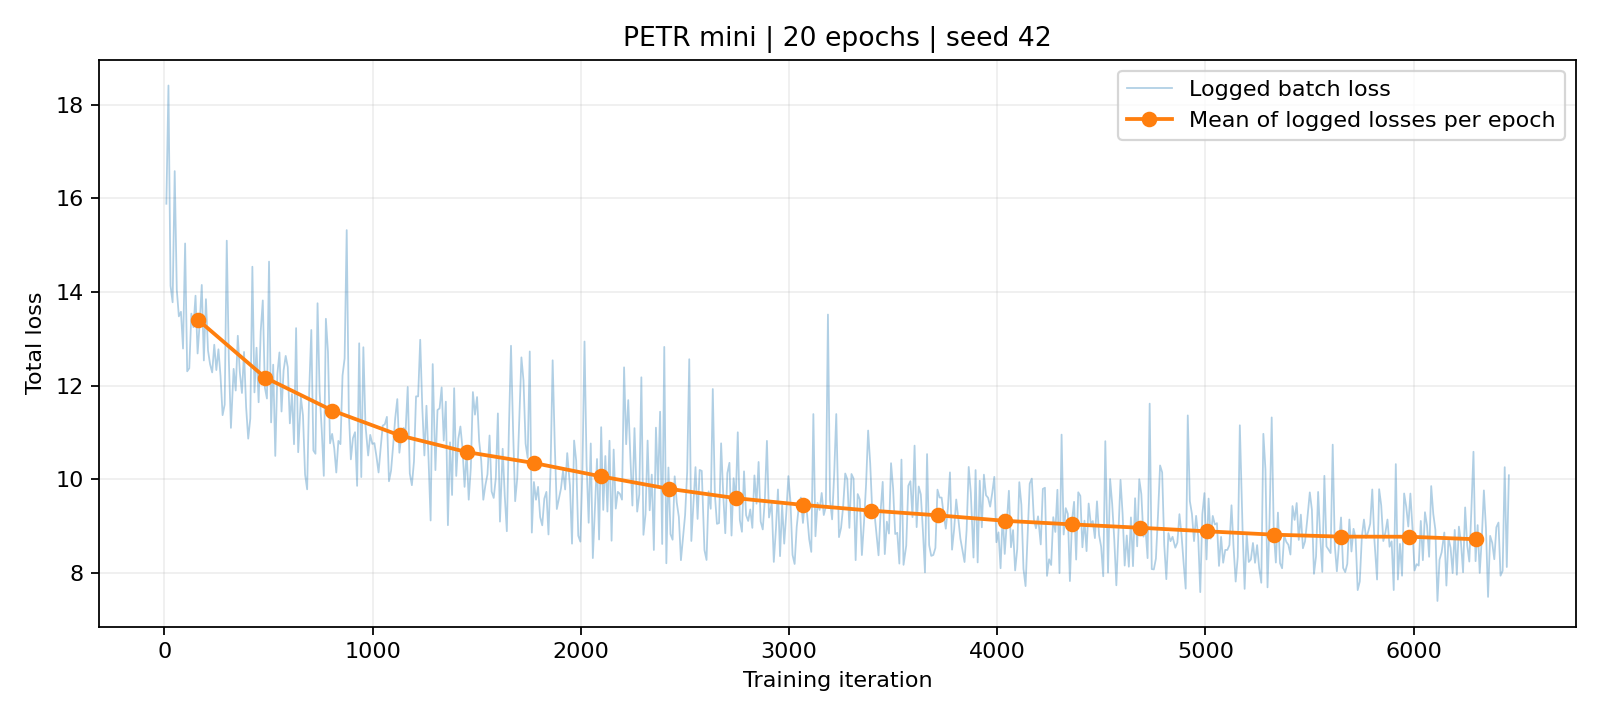
\includegraphics[width=\textwidth]{loss_curve.png}
\caption{本次 20 轮训练的总损失。浅色线为日志记录点，深色线为每轮已记录 loss 的均值。}
\label{fig:loss}
\end{figure}

\begin{table}[H]
\centering
\caption{每轮已记录批次的总损失均值}
\label{tab:loss}
\begin{tabular}{rrr@{\hspace{1.2cm}}rrr}
\toprule 轮数 & 平均 loss & 记录点 & 轮数 & 平均 loss & 记录点 \\
\midrule
1 & 13.408410 & 32 & 11 & 9.335098 & 32 \\
2 & 12.173871 & 32 & 12 & 9.233896 & 32 \\
3 & 11.469444 & 32 & 13 & 9.116602 & 32 \\
4 & 10.939249 & 32 & 14 & 9.039887 & 32 \\
5 & 10.582981 & 32 & 15 & 8.969102 & 32 \\
6 & 10.349185 & 32 & 16 & 8.892692 & 32 \\
7 & 10.062767 & 32 & 17 & 8.820684 & 32 \\
8 & 9.800701 & 32 & 18 & 8.779293 & 32 \\
9 & 9.600143 & 32 & 19 & 8.776940 & 32 \\
10 & 9.455704 & 32 & 20 & 8.723793 & 32 \\
\bottomrule
\end{tabular}
\end{table}

日志每 10 次迭代记录一次，各轮有 32 个记录点，共 640 点。表\ref{tab:loss}为这些记录点的均值，不是每轮全部 323 批次的精确平均值。已记录的 loss 均未出现 NaN/Inf；轮均值由 13.408410 降到 8.723793，下降约 34.94\%。损失下降表示训练目标被优化，仍须用验证指标判断检测能力。
\FloatBarrier

\section{全部验证帧评估与预测显示}
\Needspace{5\baselineskip}
\subsection{官方指标和类别结果}

第 20 轮权重完成全部 81 帧推理，保存原始 \path{predictions.pkl}、nuScenes 格式 \path{results_nusc.json} 和官方指标文件。输出 token 与验证索引完全对应。mini 没有本次可用的独立带标注 test 拆分，课程 \texttt{test.py} 执行的是 \texttt{mini\_val} 评估，本报告不将它称为独立测试成绩。

\begin{table}[H]
\centering
\caption{81 帧 mini\_val 的最终指标}
\label{tab:metrics}
\begin{tabular}{lrl}
\toprule 指标 & 实际值 & 含义或单位 \\
\midrule
mAP & 0.000569 & 中心距离 AP 汇总 \\
NDS & 0.028768 & 综合检测分数 \\
mATE & 1.026323 & 位置误差 / m \\
mASE & 0.926808 & 尺寸误差 \\
mAOE & 1.053263 & 朝向误差 / rad \\
mAVE & 0.897892 & 速度误差 / m/s \\
mAAE & 0.890463 & 属性误差 \\
\bottomrule
\end{tabular}
\end{table}

mAP 按 0.5、1、2、4 m 四个中心距离阈值汇总十类 AP，NDS 综合 AP 与五项误差。误差表中的尺寸和属性误差无量纲。多数类别的 TP 误差为 1.0，是评估器在召回不足时使用的默认惩罚，不能一律解释为实测每个目标误差恰好为 1。traffic\_cone 的朝向、速度、属性项以及 barrier 的速度、属性项在官方文件中为 NaN，表示不适用，与训练 loss 的 NaN 是不同概念；汇总指标均为有限值。

\begin{table}[H]
\centering
\caption{四个中心距离阈值平均后的逐类 AP}
\begin{tabular}{lr}
\toprule 类别 & AP \\
\midrule
car & 0.005690 \\
truck & 0.000000 \\
bus & 0.000000 \\
trailer & 0.000000 \\
construction\_vehicle & 0.000000 \\
pedestrian & 0.000000 \\
motorcycle & 0.000000 \\
bicycle & 0.000000 \\
traffic\_cone & 0.000000 \\
barrier & 0.000000 \\
\bottomrule
\end{tabular}
\end{table}

只有 car 在 4 m 阈值下有非零 AP，值为 0.022759；car 在 0.5、1、2 m 阈值下的 AP 均为零，其余九类 AP 均为零。验证集缺失三个类别，不能解释已有 truck、bus、pedestrian、motorcycle、bicycle、traffic\_cone 真实目标类别的零 AP。
\FloatBarrier

\Needspace{5\baselineskip}
\subsection{六相机对比图与俯视图}

本次默认选取按时间排序的前三帧，均来自 \texttt{scene-0103}。每帧先按分数阈值 0.1 筛选，再全帧共享 top-20，不是每路相机各选 20 个框。三个样本均选出了 20 个框，绘图参数与教程一致。

图\ref{fig:camera0}的上两排是绿色真实框，下两排是红色预测框，相机排列顺序一致。框由全局坐标转换到各相机坐标后按内参投影，满足角点在相机前方及图像可见性条件时绘制，同一框可能出现在多路相机。图中多个红框落在道路、建筑或栏杆区域，与可见行人及车辆不对应。

\begin{figure}[H]
\centering
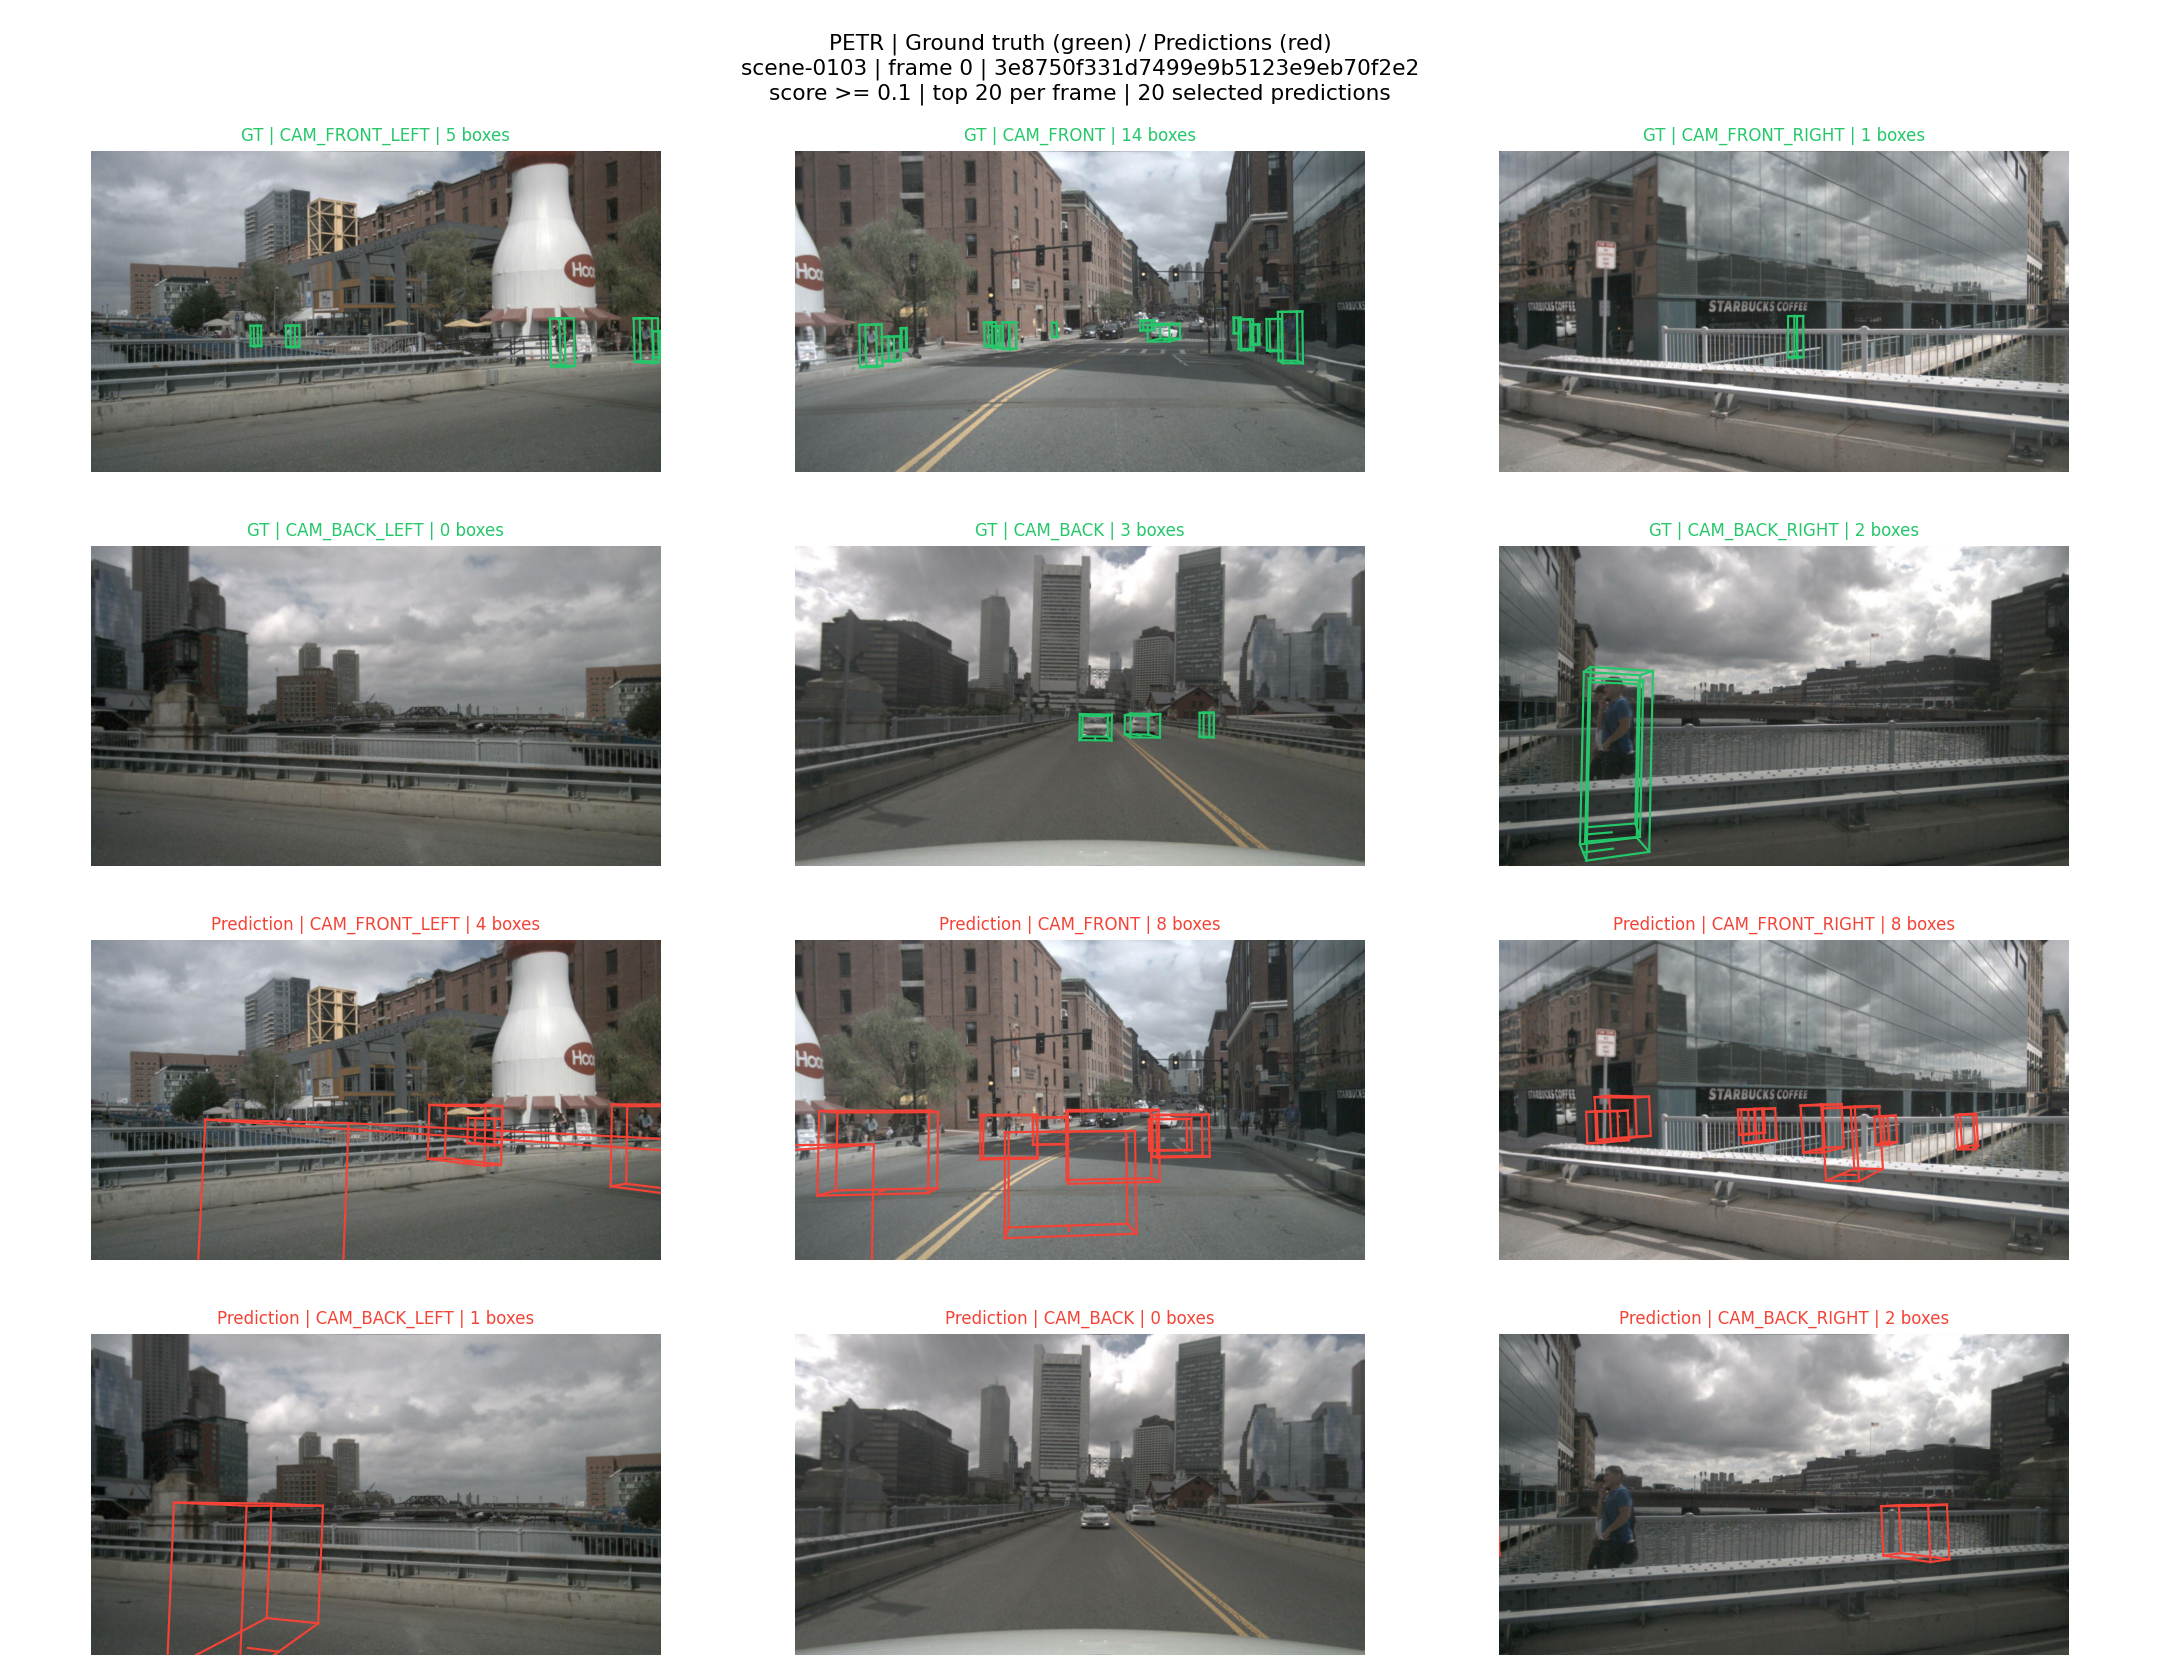
\includegraphics[width=\textwidth]{frame_000_scene-0103_cameras.png}
\caption{第 0 帧六相机真实框与预测框对比。绿色为真实框，红色为预测框；阈值 0.1，全帧 top-20。}
\label{fig:camera0}
\end{figure}

\begin{figure}[H]
\centering
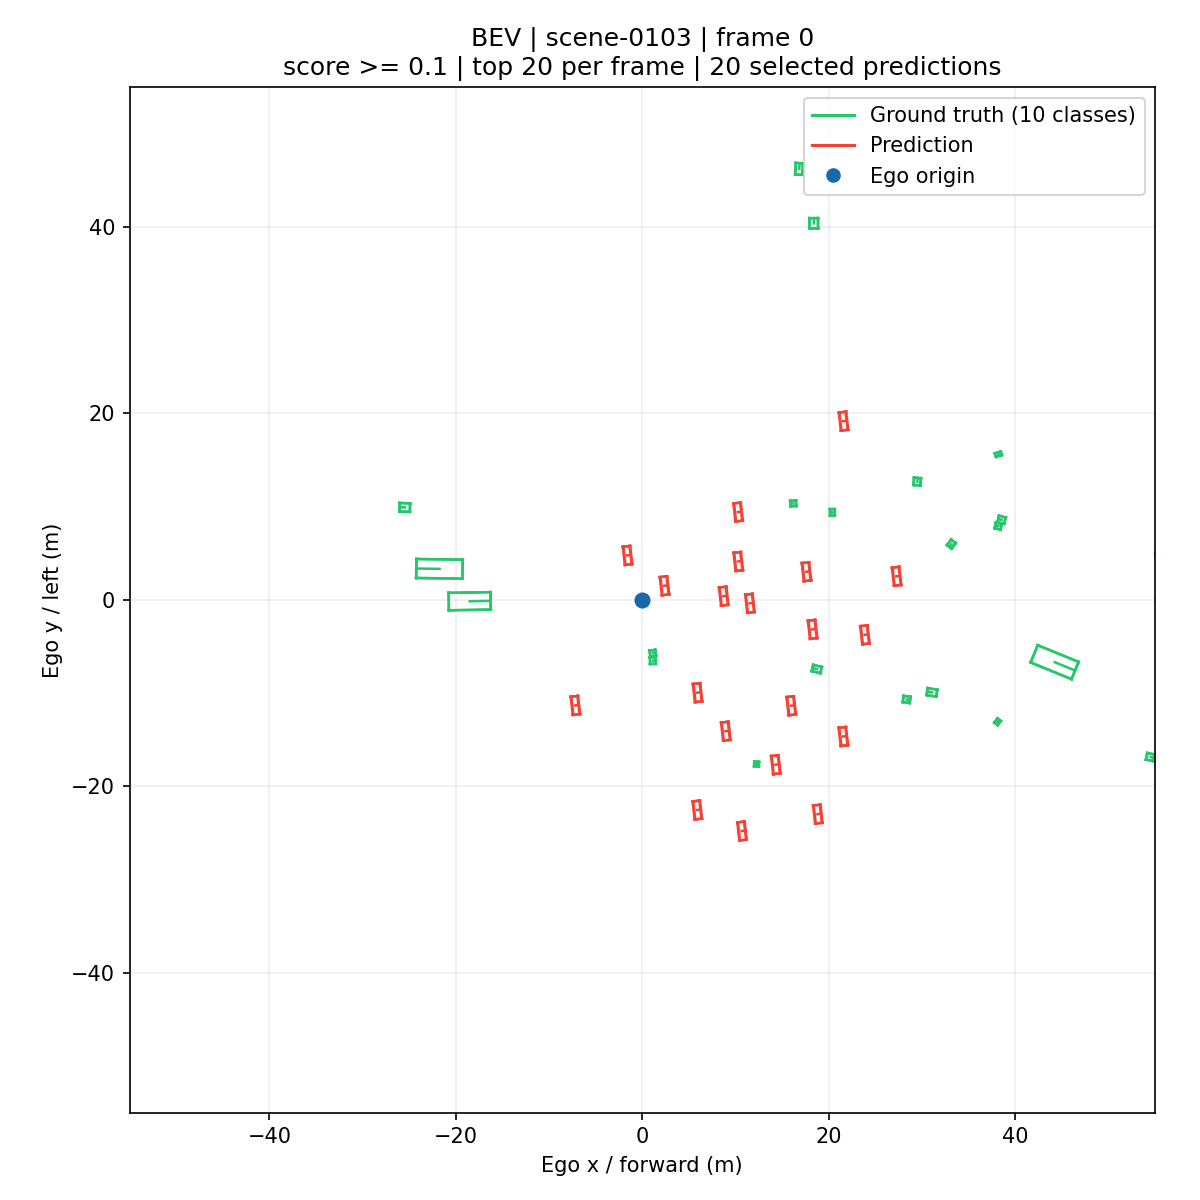
\includegraphics[width=0.75\textwidth]{frame_000_scene-0103_bev.png}
\caption{第 0 帧检测俯视图。横轴 $x$ 向前、纵轴 $y$ 向左，单位米；蓝点为前相机时刻的自车原点，范围为正负 55 m。}
\label{fig:bev0}
\end{figure}

俯视图绿色框为真实框，红色框为预测框。真实框保留十个检测类别，但没有套用评估器全部距离和点数过滤，因此图中真实框数量不必等于评估器数量。实际图中大量预测框与真实框不重合，位置、尺寸或朝向差异明显。

第 0 帧前相机有 14 个真实框、8 个预测框；后相机有 3 个真实框而所选预测无可见框。框数量接近不代表正确匹配。部分相机没有红框时，应结合 \path{visualization_info.json} 判断所选框的可见性；本次三帧都存在 20 个过阈值预测，不能把空相机视图直接归因于分数过低。其余两帧完整图见附录。
\FloatBarrier

\clearpage
\section{结果分析与实验结论}

本次训练与评估流程已经完成，但检测精度接近零。mAP=0.000569（约 0.0569\%）、NDS=0.028768（约 2.8768\%）。Loss 下降与低 AP 同时存在，说明训练误差的改善并不保证验证检测可靠。

81 帧格式化结果共有 6783 个预测框，其中 car=6319、barrier=399、pedestrian=65，其他类别没有保留预测；汽车占比约 93.16\%。预测分数为 0.232150--0.294952，中位数 0.290025，全部高于展示阈值 0.1。输出明显偏向汽车，降低绘图阈值不能解决错误位置、类别或提高 AP。

训练集只有 323 帧，验证类别覆盖不完整，同时使用较低分辨率及缩小模型，这些都是教学实验限制。但仅凭本次结果不能确认低精度的主要原因，也不能直接断言存在坐标变换程序错误。后续可以核对图像增强与标定、框编码与解码的一致性，分析逐类训练信号，并进行单帧拟合实验；这些是进一步排查建议，本报告不把未执行的实验当成已得到的证据。

本次完成了六相机统一坐标显示、PETR 关键代码阅读、20 轮训练、全部 81 帧评估和三帧默认可视化。已检查最终权重、已记录 loss、结果 token、图片与显示参数，所有流程验收项通过；模型检测效果很差，尚不能作为可靠的三维检测模型。

\subsection*{依据与复现材料}
课程《PETR实践指导文档》；本地 PETR 插件与教学配置；本次 \path{outputs/run20/20260929_153058.log} 和结构化日志；\path{epoch_loss_summary.json}；\path{metrics_summary.json}；\path{visualization_info.json}；\path{six_camera_calibration.json}；\path{prediction_stats.json} 及 \path{experiment_validation.json}。提交包中的 README 说明依赖、数据与权重准备、运行命令；报告源文件和编译辅助文件仅在本地保留。

\clearpage
\appendix
\section{其余两帧的完整预测可视化}

以下图片沿用正文相同的真实框/预测框颜色、阈值 0.1、全帧 top-20 和俯视坐标说明。图中预测与目标的错位在相邻帧仍然存在。

\begin{figure}[H]
\centering
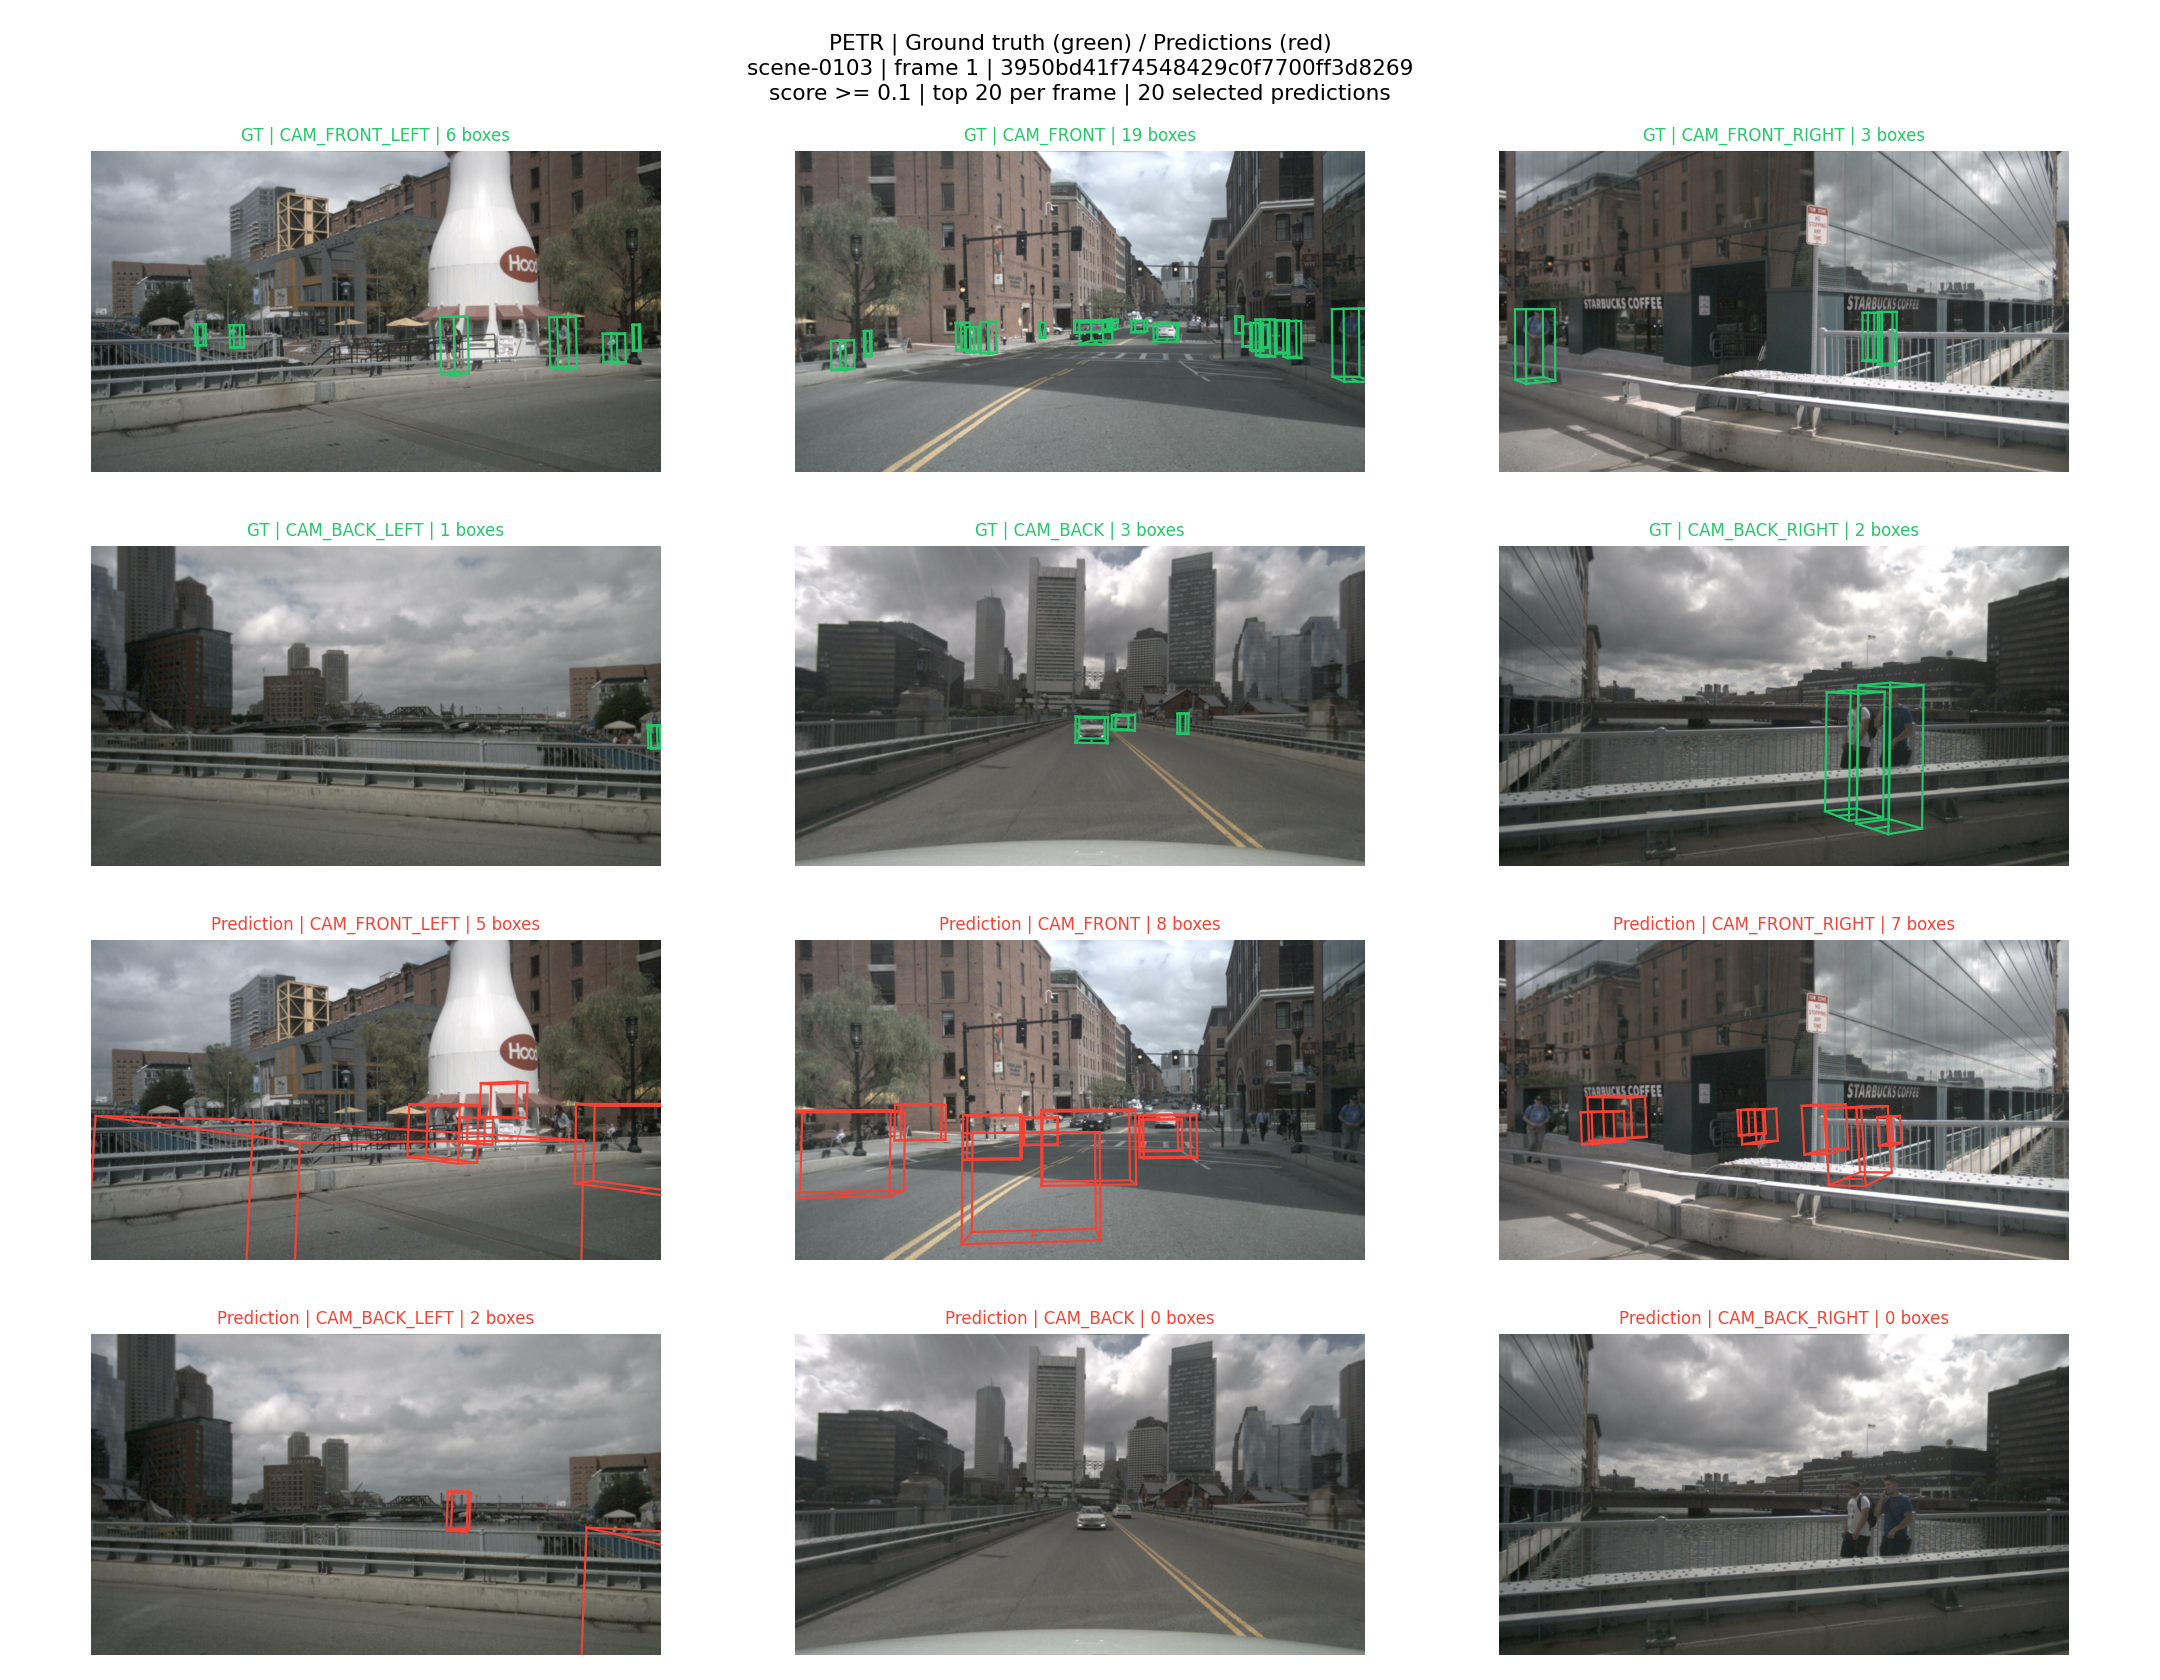
\includegraphics[width=\textwidth]{frame_001_scene-0103_cameras.png}
\caption{第 1 帧六相机真实框与预测框对比。}
\end{figure}
\begin{figure}[H]
\centering
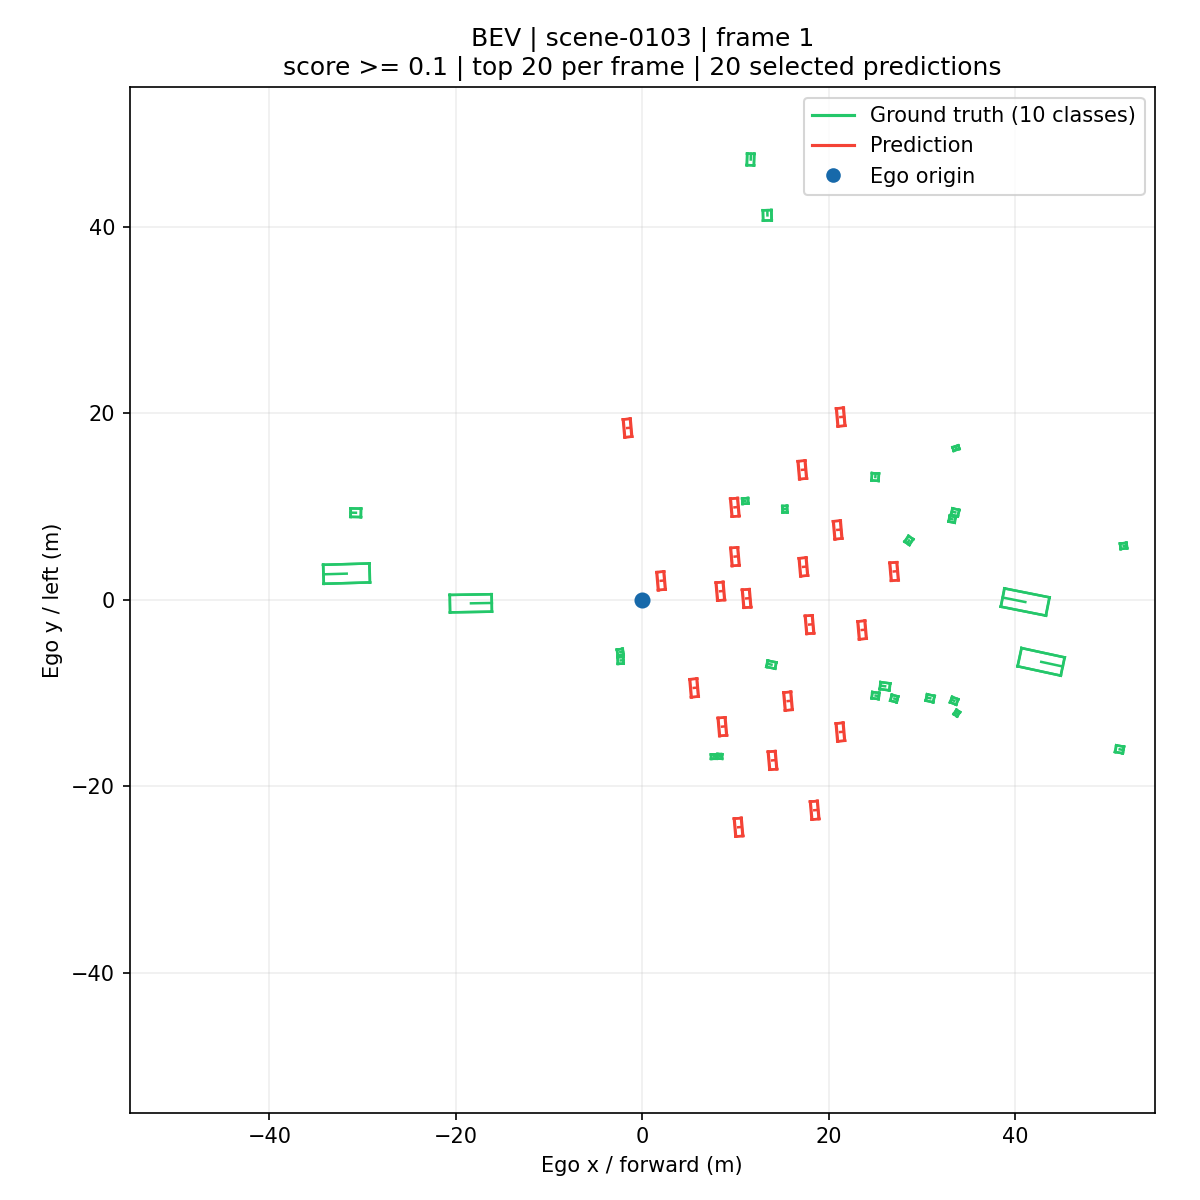
\includegraphics[width=0.74\textwidth]{frame_001_scene-0103_bev.png}
\caption{第 1 帧俯视图，单位米；绿色真实框，红色预测框，蓝色自车原点。}
\end{figure}
\FloatBarrier
\begin{figure}[H]
\centering
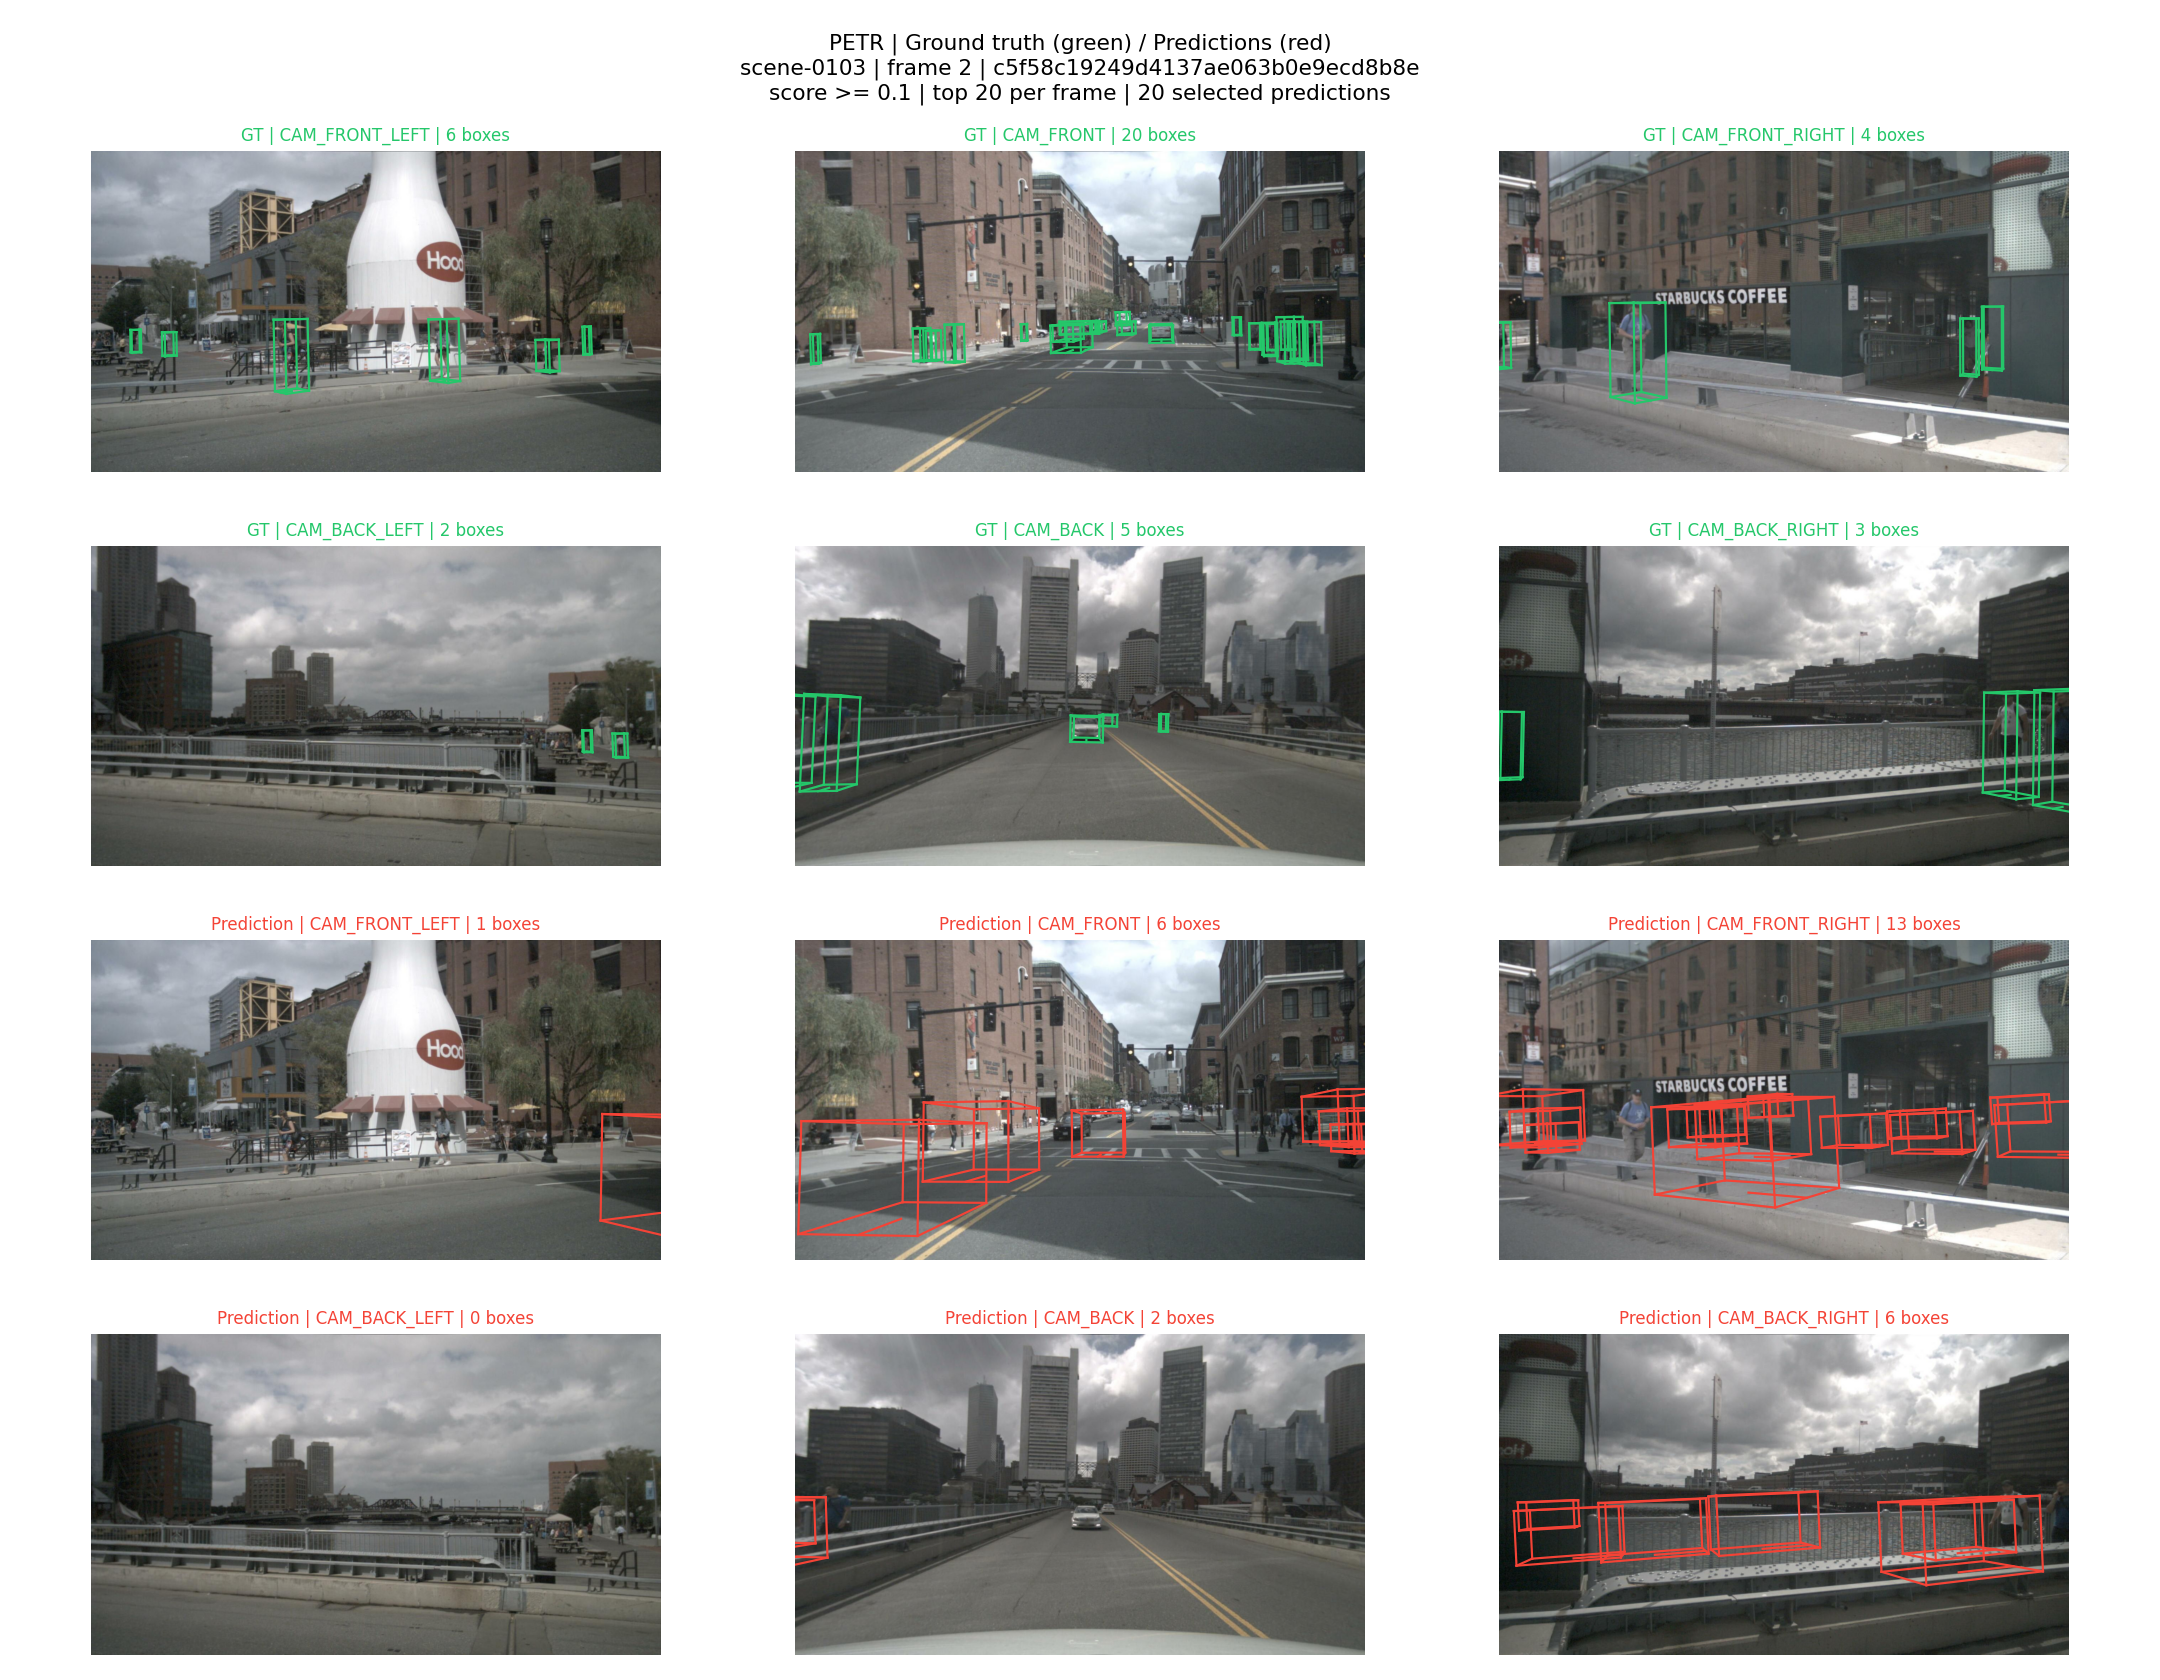
\includegraphics[width=\textwidth]{frame_002_scene-0103_cameras.png}
\caption{第 2 帧六相机真实框与预测框对比。}
\end{figure}
\begin{figure}[H]
\centering
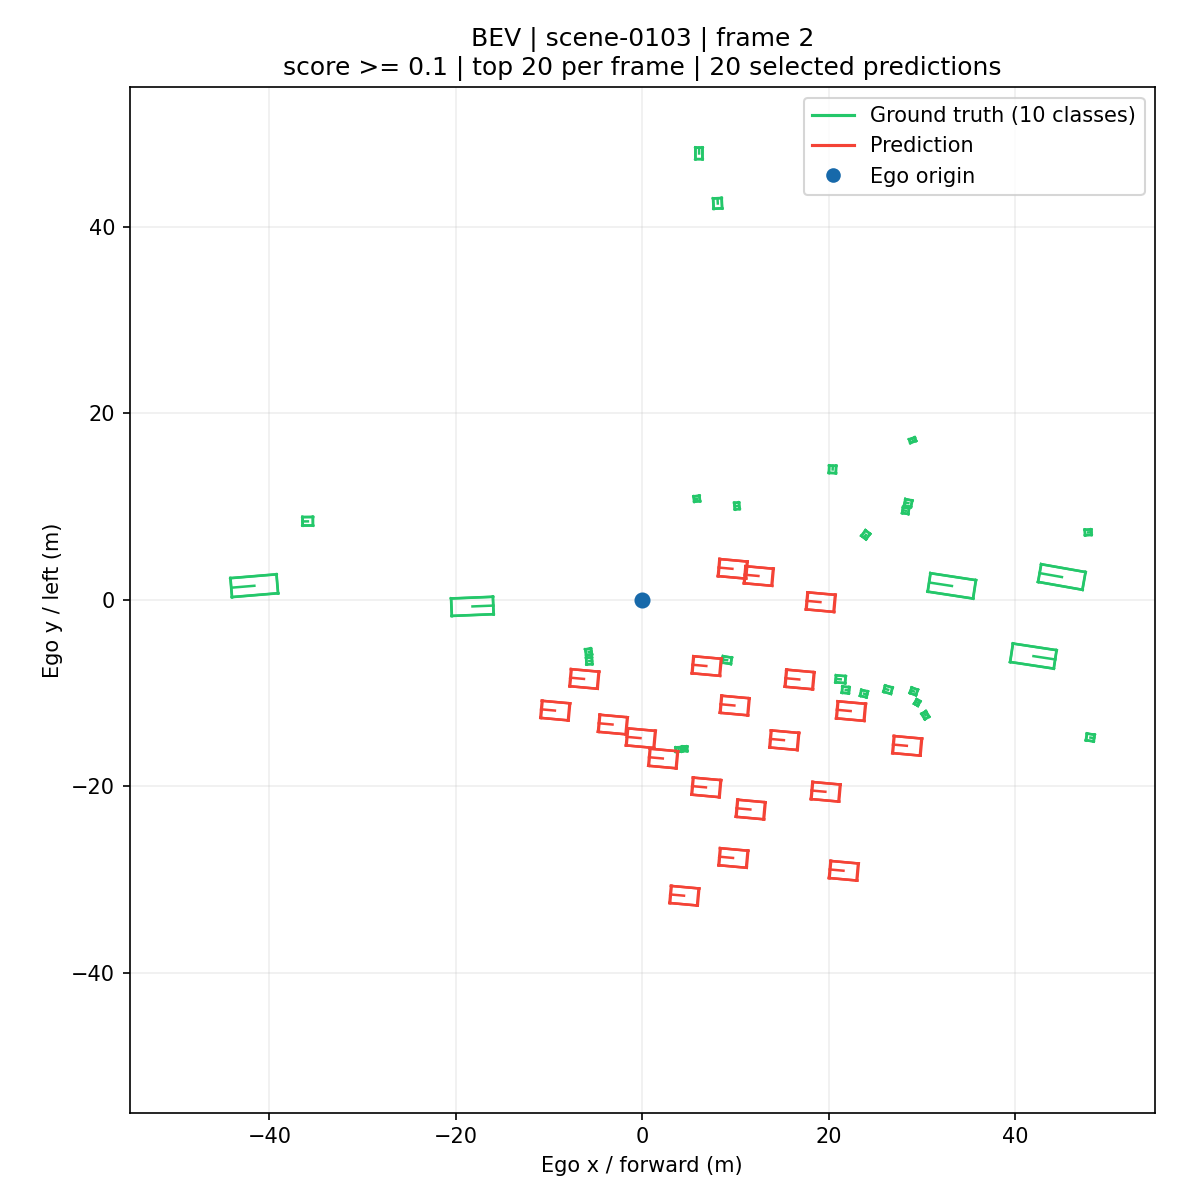
\includegraphics[width=0.74\textwidth]{frame_002_scene-0103_bev.png}
\caption{第 2 帧俯视图，单位米；绿色真实框，红色预测框，蓝色自车原点。}
\end{figure}
\FloatBarrier
\end{document}
